\documentclass{article}
\usepackage[utf8]{inputenc}
\usepackage{amsmath}
\usepackage{amssymb}
\usepackage{graphicx}
\usepackage{xcolor}



\begin{document}
\section*{QR-Factorization of Tridiagonal Matrices}

\subsection*{3-4.a} 
We are tasked with proving that for a \textbf{tridiagonal} invertible matrix $\mathbf{A} \in \mathbb{R}^{n,n}$ a QR-factorization $\mathbf{A}= \mathbf{Q}\mathbf{R}$, $\mathbf{Q}\in \mathbb{R}^{n,n}$ orthogonal, $\mathbf{R}\in \mathbb{R}^{n,n}$ upper triangular with positive diagonal entries, satisfies
\begin{equation*}
    \left(\mathbf{R}\right)_{i,j} = 0 \text{ for } j > i + 2 \:\text{ and }\: \left(\mathbf{Q}\right)_{i,j} = 0 \text{ for } i > j + 1
\end{equation*}
We know little about the structure of $\mathbf{Q}$, but we do know quite a lot about the structure of $\mathbf{A}$ and $\mathbf{R}$. We now remember the following lemma from the lecture document.

\begin{figure}[!hbt]
    \centering
\includegraphics[width=1.0\linewidth]{StructureOfInvertedMatrix.png}
\end{figure}

\noindent We can hence state that because $\mathbf{R}$ is upper triangular with positive diagonal entries (it has thus a positive determinant) that it must be regular and because of the above lemma $\mathbf{R}^{-1}$ must also be upper triangular. We can thus write $\mathbf{Q} = \mathbf{A}\mathbf{R}^{-1}$. Let us look at this product. Let us denote $\mathbf{R}^{-1} = \mathbf{S}$, we then consider the following sum.
\begin{align*}
    \left(\mathbf{Q}\right)_{i,j} = \left(\mathbf{A}\mathbf{S}\right)_{i,j} = \sum_{l=1}^{n}a_{il}s_{lj}
\end{align*}
Let us first visualize the situation for a simple example.
\begin{equation*}
    \begin{bmatrix}
        a_{11} & a_{12} & 0 & 0 & 0\\
        a_{21} & a_{22} & a_{23} & 0 & 0 \\
        0 & a_{32} & a_{33} & a_{34} & 0 \\
        0 & 0 & a_{43} & a_{44} & a_{45} \\
        0 & 0 & 0 & a_{54} & a_{55}
    \end{bmatrix}
    \begin{bmatrix}
        s_{11} & s_{12} & s_{13} & s_{14} & s_{15} \\
        0 & s_{22} & s_{23} & s_{24} & s_{25} \\
        0 & 0 & s_{33} & s_{34} & s_{35} \\
        0 & 0 & 0 & s_{44} & s_{45} \\
        0 & 0 & 0 & 0 & s_{55}
    \end{bmatrix} = 
    \begin{bmatrix}
        \star & \star & \star & \star & \star \\
        \star & \star & \star & \star & \star \\
        0 & \star & \star & \star & \star \\
        0 & 0 & \star & \star & \star \\
        0 & 0 & 0& \star & \star
    \end{bmatrix}
\end{equation*}
We hence can see that the zero entries of the result matrix will be were the lower triangular part of $\mathbf{A}$ has zero entries. This translates to
\begin{align*}
   \left(\mathbf{Q}\right)_{i,j} = \sum_{l=1}^{n}a_{il}s_{lj} = \sum_{l \in \left\{i - 1, i, i+1\right\}} a_{il}s_{lj} \quad \text{($a_{il} = 0 \text{ for } i < l - 1$ and $i > l + 1$)}
\end{align*}
Using that $\mathbf{S}$ is upper triangular we can see that we have
\begin{equation*}
    \left(\mathbf{Q}\right)_{i,j} = \sum_{l \in \left\{i - 1, i, i+1\right\}, l \leq j} a_{il}s_{lj}
\end{equation*}
For this term to be zero, we must make is such that the two conditions exclude each other. This is the case when $l \geq i - 1$ makes $l \leq j$ impossible, which happens for $i - 1 > j$ and hence for $i > j + 1$. We hence write
\begin{equation}
    \left(\mathbf{Q}\right)_{i,j} = 0 \text{ if } i > j + 1
\end{equation}

\noindent We now use that $\mathbf{Q}$ is orthogonal and thus we have $\mathbf{Q}^{-1} = \mathbf{Q}^{\mathsf{T}}$. We can use this as it gives us $\mathbf{R} = \mathbf{Q}^{\mathsf{T}}\mathbf{A}$. We again first illustrate this in a small example, here we us that we have derived (1) already and hence we know that some of the entries of $\mathbf{Q}$ must be $0$.
\begin{equation*}
    \begin{bmatrix}
        q_{11} & q_{21}  & 0 & 0 & 0 \\
        q_{12} & q_{22} & q_{23} & 0 & 0 \\
        q_{13} & q_{23} & q_{33} & q_{43} & 0 \\
        q_{14} & q_{24} & q_{34} & q_{44} & q_{54} \\
        q_{15} & q_{25} & q_{35} & q_{45} & q_{55}
    \end{bmatrix}
    \begin{bmatrix}
        a_{11} & a_{12} & 0 & 0 & 0\\
        a_{21} & a_{22} & a_{23} & 0 & 0 \\
        0 & a_{32} & a_{33} & a_{34} & 0 \\
        0 & 0 & a_{43} & a_{44} & a_{45} \\
        0 & 0 & 0 & a_{54} & a_{55}
    \end{bmatrix}
    = \begin{bmatrix}
        \star & \star & \star & 0 & 0 \\
        \mathbf{0} & \star& \star & \star & 0 \\
        \mathbf{0} & \mathbf{0} & \star & \star & \star \\
        \mathbf{0} & \mathbf{0} & \mathbf{0} & \star &\star \\
        \mathbf{0} & \mathbf{0} & \mathbf{0} & \mathbf{0} & \star
    \end{bmatrix}
\end{equation*}
Here the zero entries $\mathbf{0}$ are zero, because the result is an upper triangular matrix ($\mathbf{R}$), the other zero entries are because of $(1)$. Mathematically we can write this as
\begin{align*}
\left(\mathbf{Q}^{\mathsf{T}}\mathbf{A}\right)_{i,j} = \sum_{l=1}^{n}\left(\mathbf{Q}^{\mathsf{T}}\right)_{i,l}a_{lj} &= \sum_{l=1}^{n}q_{li}a_{lj} \\
&= \sum_{l \in \left\{j-1,j,j+1\right\}}q_{li}a_{lj} \quad \text{($\mathbf{A}$ is tridiagonal)} \\
&= \sum_{l \in \left\{j-1,j,j+1\right\}, l \leq i + 1}q_{li}a_{lj} \quad \text{(1)}
\end{align*}
Here we get that the sum is zero if $l \geq j - 1$ makes $l \leq i +1$ impossible, hence we get $j - 1 > i + 1$ and thus $j > i + 2$. Which gives us
\begin{equation}
    \left(\mathbf{R}\right)_{i,j} = 0 \text{ if } j > i + 2
\end{equation} 
Hence with (1) and (2) both equations in (3.4.1) have been shown.

\pagebreak

\subsection*{3-4.b}

\noindent To store a QR-Factorization $\mathbf{A} = \mathbf{Q}\mathbf{R}$ of a real-valued \textbf{tridiagonal} matrix $\mathbf{A}\in \mathbb{R}^{n,n}$ we use the following data structure.

\begin{figure}[!hbt]
    \centering
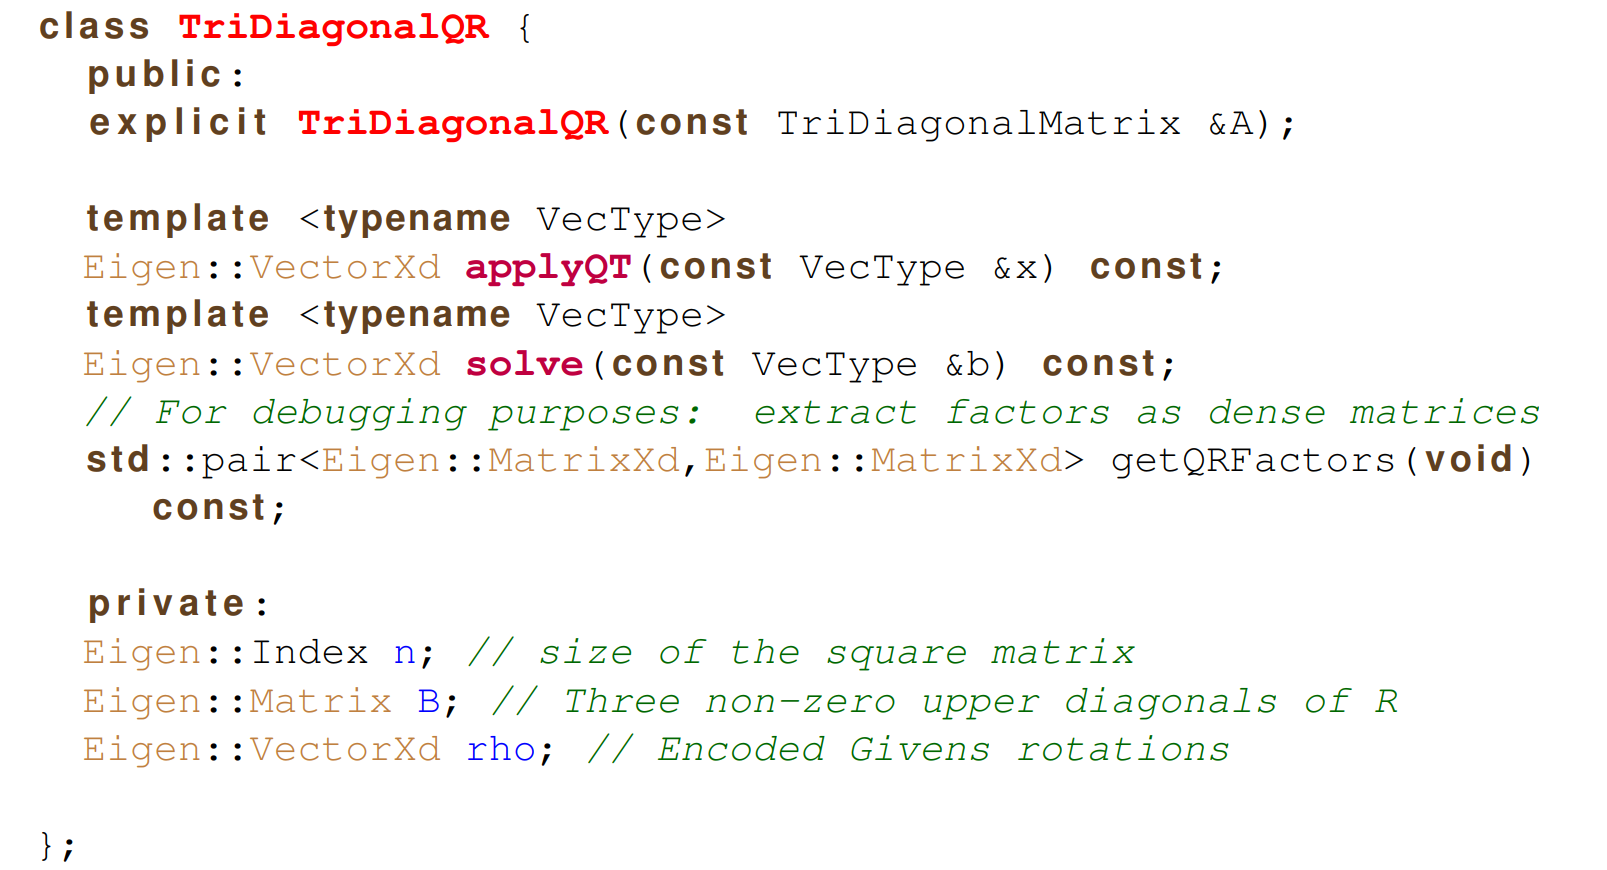
\includegraphics[width=1.0\linewidth]{3-4CodeDef.png}
\end{figure}

\noindent For the matrix $\mathbf{B}$ we use the following storage format, where all entries of $\mathbf{R}$ are stored in $\mathbf{B}$.
\begin{figure}[!hbt]
    \centering
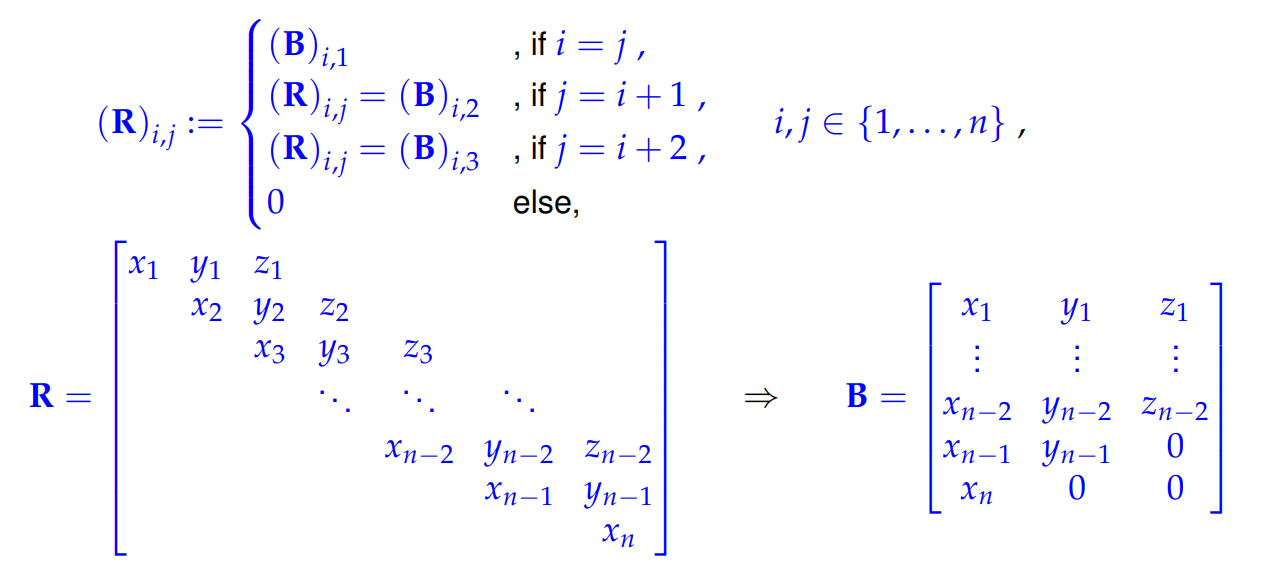
\includegraphics[width=0.7\linewidth]{3-4MatrixDef.png}
\end{figure}

\noindent The $\mathbf{Q}$ matrix is stored in compressed format through $n-1$ underlying Givens rotations. Every Givens rotation is stored through a single number $\rho$.
\begin{figure}[!hbt]
    \centering
\includegraphics[width=0.7\linewidth]{RhoEncodingGivens.png}
\end{figure}


 \noindent We are now tasked with implementing a function \verb|compGivensRotation| that computes a Givens rotation mapping the vector $\mathbf{a} \in \mathbb{R}^{2}$ onto a multiple of the first Cartesian coordinate vector $\mathbf{e}_{1}\in \mathbb{R}^{2}$. We will for this purpose use the equations given to us in the lecture document under section 3.3.3.15.
\begin{equation*}
    \gamma = \frac{a_{1}}{\sqrt{\left\lvert a_{1}\right\rvert^{2} + \left\lvert a_{k} \right\rvert^{2}}} \qquad \sigma= \frac{a_{k}}{\sqrt{\left\lvert a_{1}\right\rvert^{2} + \left\lvert a_{k} \right\rvert^{2}}}
\end{equation*}
We know think back to Problem 1.8, in which we discussed the problematic of computing squares of numbers and how both overflow and underflow can occur when doing the computation. We start with the $\gamma$ term. We can write (we assume that $a_{k} \neq 0$ and treat this case separately in our code)
\begin{equation*}
    \gamma = \frac{a_{1}}{\sqrt{\left\lvert a_{1}\right\rvert^{2} + \left\lvert a_{k} \right\rvert^{2}}} =\frac{a_{1}}{\sqrt{ a_{1}^{2} + a_{k}^{2}}} =\frac{a_{1}}{\sqrt{\frac{a_{1}^{2}\left(a_{1}^{2} +  a_{k}^{2}\right)}{a_{1}^{2}}}} = \frac{a_{1}}{\sqrt{a_{1}^{2}}\sqrt{\frac{a_{1}^{2} +  a_{k}^{2}}{a_{1}^{2}}}} =  \frac{a_{1}}{a_{1}\sqrt{\frac{a_{1}^{2} +  a_{k}^{2}}{a_{1}^{2}}}}
\end{equation*}
which gives us
\begin{equation*}
    \gamma = \frac{1}{\sqrt{\frac{a_{1}^{2} +  a_{k}^{2}}{a_{1}^{2}}}} = \frac{1}{\sqrt{1 + \frac{a_{k}^{2}}{a_{1}^{2}}}} = \frac{1}{\sqrt{1 + \left(\frac{a_{k}}{a_{1}}\right)^{2}}}
\end{equation*}
For $\sigma$ we get 
\begin{equation*}
    \sigma = \frac{a_{k}}{\sqrt{\left\lvert a_{1}\right\rvert^{2} + \left\lvert a_{k} \right\rvert^{2}}} =\frac{a_{k}}{\sqrt{ a_{1}^{2} + a_{k}^{2}}} =\frac{a_{k}}{\sqrt{\frac{a_{k}^{2}\left(a_{1}^{2} +  a_{k}^{2}\right)}{a_{k}^{2}}}} = \frac{a_{k}}{\sqrt{a_{k}^{2}}\sqrt{\frac{a_{1}^{2} +  a_{k}^{2}}{a_{k}^{2}}}} =  \frac{a_{k}}{a_{k}\sqrt{\frac{a_{1}^{2} +  a_{k}^{2}}{a_{1}^{2}}}}
\end{equation*}
which give us
\begin{equation*}
    \sigma = \frac{1}{\sqrt{\frac{a_{1}^{2} + a_{k}^{2}}{a_{k}^{2}}}} = \frac{1}{\sqrt{1 + \frac{a_{1}^{2}}{a_{k}^{2}}}} = \frac{1}{\sqrt{1 + \left(\frac{a_{1}}{a_{k}}\right)^{2}}}
\end{equation*}
Keep in mind that this works only in the 2D case, as otherwise instead of the absolute value we would have the norm, which would not allow for us to do steps made above. Now to avoid overflow we distinguish two cases  for $\mathbf{a} = \left[a_{0}, a_{1}\right]^{\mathsf{T}}$.
\paragraph{Case $\left\lvert a_{1}\right\rvert \geq \left\lvert a_{0}\right\rvert$:} Here we set $t = -\frac{a_{0}}{a_{1}}$, $\sigma = \frac{1}{\sqrt{1 + t^{2}}}$ and $\gamma = \sigma t$, we verify
\begin{align*}
    \begin{bmatrix}
    \gamma & \sigma \\
    -\sigma & \gamma
    \end{bmatrix}^{\mathsf{T}}\begin{bmatrix}
        a_{0} \\ a_{1}
    \end{bmatrix} &= \begin{bmatrix}
        \gamma a_{0} - \sigma a_{1} \\
        \sigma a_{0} + \gamma a_{1}
    \end{bmatrix} = \begin{bmatrix}
        \sigma t a_{0} - \sigma a_{1} \\
        \sigma a_{0} + \sigma t a_{1}
    \end{bmatrix} = \sigma \begin{bmatrix}
        t a_{0} - a_{1} \\
        a_{0} + t a_{1}
    \end{bmatrix} \\[1mm]
    &= \frac{a_{1}}{\sqrt{a_{0}^{2} +a_{1}^{2}}}\begin{bmatrix}
        -\frac{a_{0}^{2}}{a_{1}} - a_{1} \\
        a_{0} - \frac{a_{1}a_{0}}{a_{1}}
    \end{bmatrix} = \frac{a_{1}}{\sqrt{a_{0}^{2} +a_{1}^{2}}}\begin{bmatrix}
        -\frac{a_{0}^{2} + a_{1}^{2}}{a_{1}} \\
        a_{0} - a_{0}
    \end{bmatrix}
\end{align*}

\pagebreak

\noindent which then leads to
\begin{equation*}
     \frac{a_{1}}{\sqrt{a_{0}^{2} +a_{1}^{2}}}\begin{bmatrix}
        -\frac{a_{0}^{2} + a_{1}^{2}}{a_{1}} \\
        a_{0} - a_{0}
    \end{bmatrix}  = \frac{a_{1}}{\left\lVert \mathbf{a} \right\rVert_{2}}\begin{bmatrix}
        -\frac{\left\lVert \mathbf{a} \right\rVert_{2}^{2}}{a_{1}} \\
        0
    \end{bmatrix} =
    \begin{bmatrix}
   -\left\lVert \mathbf{a} \right\rVert_{2} \\
        0
    \end{bmatrix}
\end{equation*}
\paragraph{Case $\left\lvert a_{1}\right\rvert < \left\lvert a_{0}\right\rvert$:} Here we set $t = -\frac{a_{1}}{a_{0}}$, $\gamma = \frac{1}{\sqrt{1 + t^{2}}}$ and $\sigma = \gamma t$, we verify
\begin{align*}
    \begin{bmatrix}
    \gamma & \sigma \\
    -\sigma & \gamma
    \end{bmatrix}^{\mathsf{T}}\begin{bmatrix}
        a_{0} \\ a_{1}
    \end{bmatrix} &= \begin{bmatrix}
        \gamma a_{0} - \sigma a_{1} \\
        \sigma a_{0} + \gamma a_{1}
    \end{bmatrix} =
    \begin{bmatrix}
        \gamma a_{0} - \gamma t a_{1} \\
        \gamma t a_{0} + \gamma a_{1}
    \end{bmatrix} =\gamma \begin{bmatrix}
        a_{0} - t a_{1} \\
        ta_{0} + a_{1}
    \end{bmatrix} \\ &= 
    \frac{a_{0}}{\sqrt{a_{0}^{2} + a_{1}^{2}}}
    \begin{bmatrix}
        a_{0} + \frac{a_{1}^{2}}{a_{0}}  \\
        -\frac{a_{0}a_{1}}{a_{0}} + a_{1}
    \end{bmatrix} =
    \frac{a_{0}}{\left\lVert \mathbf{a}\right\rVert_{2}} \begin{bmatrix}
 \frac{a_{0}^{2} + a_{1}^{2}}{a_{0}}  \\
        -a_{1} + a_{1}
    \end{bmatrix} \\
    &= \frac{a_{0}}{\left\lVert \mathbf{a}\right\rVert_{2}} \begin{bmatrix}
 \frac{\left\lVert \mathbf{a}\right\rVert_{2}^{2}}{a_{0}}  \\
        0
    \end{bmatrix} = \begin{bmatrix}
        \left\lVert \mathbf{a}\right\rVert_{2} \\ 0
    \end{bmatrix}
\end{align*}
Hence let us actually implement this, using the case distinction and where we use one of the formulae
\begin{equation*}
    \gamma =  \frac{1}{\sqrt{1 + \left(\frac{a_{k}}{a_{1}}\right)^{2}}} \qquad \sigma = \frac{1}{\sqrt{1 + \left(\frac{a_{1}}{a_{k}}\right)^{2}}}
\end{equation*}
and the definition of $\rho$ above on the first page. This definition is different from the old one and hence one does not pass the tests anymore, but the implementation should remain correct. The code below is the result
\begin{figure}[!hbt]
    \centering
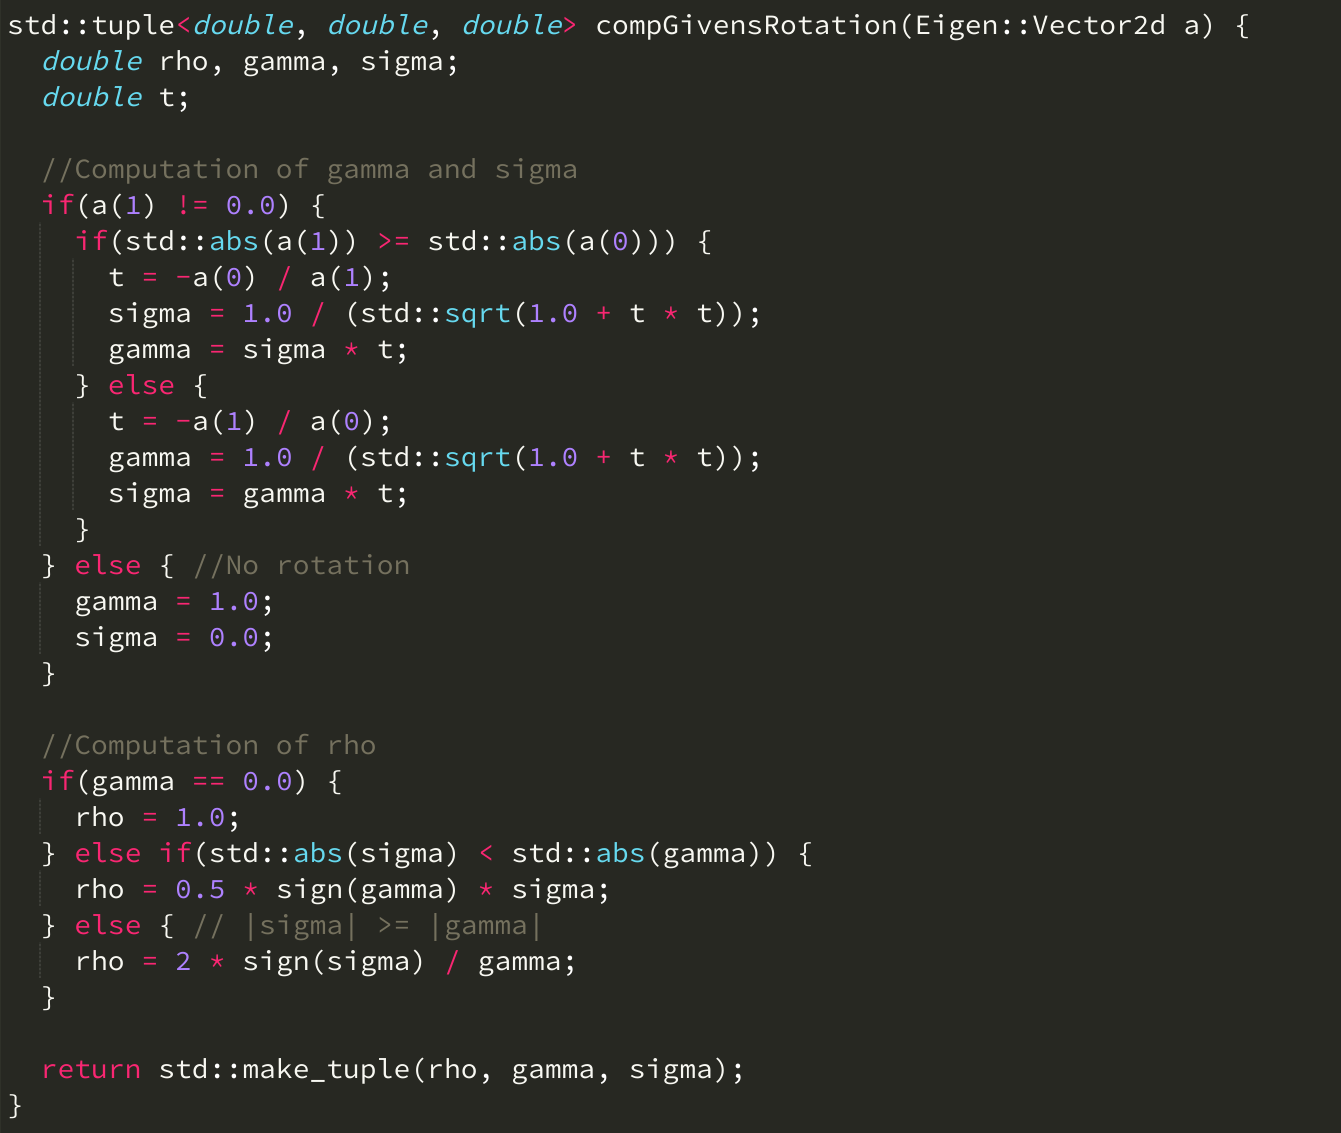
\includegraphics[width=0.8\linewidth]{3-4.a.png}
\end{figure}

\pagebreak

\noindent This implementation does not pass all the tests, as it uses a different computation of $\rho$ (the new one), with the old one (which will allow you to pass all the tests) the computation of $\rho$ would look like
\begin{figure}[!hbt]
    \centering
\includegraphics[width=0.7\linewidth]{RhoComputationOld.png}
\end{figure}

\subsection*{3-4.c}
We are now tasked with implementing an efficient code that constructs the matrix $\mathbf{R}$ of the tridiagonal matrix $\mathbf{A} \in \mathbb{R}^{n,n}$ passed to us in \verb|A|. We first need to notice the special structure of $\mathbf{R}$, this is very important, as will choose the Givens-Rotations according to this structure. $\mathbf{R}$ will have the following structure.
\begin{equation*}
\mathbf{R} =
    \begin{bmatrix}
        \star & \star & \star & 0 & 0 & 0 & 0 & 0 \\
        0 & \star & \star & \star & 0 & 0 & 0 & 0 \\
        0 & 0 & \star & \star & \star & 0 & 0 & 0 \\
        0 & 0 & 0 & \star & \star & \star & 0 & 0 \\
         0 & 0 & 0 & 0 & \star & \star & \star & 0 \\
         0 & 0 & 0 & 0 & 0 & \star & \star & \star \\
         0 & 0 & 0 & 0 & 0 & 0& \star & \star \\
         0 & 0 & 0 & 0 & 0 & 0& 0 & \star \\
    \end{bmatrix}
\end{equation*}
We know that $\mathbf{A}$ has the following structure
\begin{equation*}
    \mathbf{A} = 
    \begin{bmatrix}
    \star & \star &0 & 0 & 0 & 0 & 0 & 0 \\
        \star & \star & \star & 0& 0 & 0 & 0 & 0 \\
        0 & \star & \star & \star & 0 & 0 & 0 & 0 \\
        0 & 0 & \star & \star & \star & 0 & 0 & 0 \\
         0 & 0 & 0 & \star & \star & \star & 0  & 0 \\
         0 & 0 & 0 & 0 & \star & \star & \star & 0\\
         0 & 0 & 0 & 0 & 0 & \star& \star & \star \\
         0 & 0 & 0 & 0 & 0 & 0& \star & \star \\
    \end{bmatrix}
\end{equation*}
We get $\mathbf{R}$ from performing the Givens-Rotations on $\mathbf{A}$, we are given all the parameters to the Givens-Rotations and we know that we have $n-1$ of them. Hence we must now figure out how to apply these to go from the structure of $\mathbf{A}$ to the structure of $\mathbf{R}$. We have seen how the Givens-rotation takes annihilates the bottom row of a vector and changes the top row to the norm of the vector, using both the already partially implemented code and the fact that we are given $n-1$ Givens rotations we can guess that applying the rotations to singular vectors will not allow us to do the wished for structure change.

\pagebreak

\noindent We will now look at the what we would want our first rotation to achieve
\begin{equation*}
    \begin{bmatrix}
    \star & \star &\color{green} 0 \color{black} & 0 & 0 & 0 & 0 & 0 \\
        \color{red}\star\color{green} & \star & \star & 0& 0 & 0 & 0 & 0 \\
        0 & \star & \star & \star & 0 & 0 & 0 & 0 \\
        0 & 0 & \star & \star & \star & 0 & 0 & 0 \\
         0 & 0 & 0 & \star & \star & \star & 0  & 0 \\
         0 & 0 & 0 & 0 & \star & \star & \star & 0\\
         0 & 0 & 0 & 0 & 0 & \star& \star & \star \\
         0 & 0 & 0 & 0 & 0 & 0& \star & \star \\
    \end{bmatrix}
    \overset{G_{12}^{\mathsf{T}}}{\longrightarrow}
        \begin{bmatrix}
    \star & \star &\color{green} \star \color{black} & 0 & 0 & 0 & 0 & 0 \\
        \color{red}0\color{green} & \star & \star & 0& 0 & 0 & 0 & 0 \\
        0 & \star & \star & \star & 0 & 0 & 0 & 0 \\
        0 & 0 & \star & \star & \star & 0 & 0 & 0 \\
         0 & 0 & 0 & \star & \star & \star & 0  & 0 \\
         0 & 0 & 0 & 0 & \star & \star & \star & 0\\
         0 & 0 & 0 & 0 & 0 & \star& \star & \star \\
         0 & 0 & 0 & 0 & 0 & 0& \star & \star \\
    \end{bmatrix}
\end{equation*}
This is achieved by doing the following multiplication
\begin{equation*}
    \begin{bmatrix}
        \gamma & \sigma \\
        -\sigma & \gamma 
    \end{bmatrix}^{\mathsf{T}}
    \begin{bmatrix}
        \star & \star &\color{green} 0 \\
        \color{red} \star \color{black} & \star & \star
    \end{bmatrix}
    =
    \begin{bmatrix}
        \star & \star &\color{green} \star \color{black} \\
         \color{red}0\color{green} & \star & \star
    \end{bmatrix}
\end{equation*}
The next rotation is given to us via
\begin{equation*}
    \begin{bmatrix}
    \star & \star & \star  & 0 & 0 & 0 & 0 & 0 \\
        0& \star & \star & \color{green} 0 \color{black}& 0 & 0 & 0 & 0 \\
        0 & \color{red}\star \color{black} & \star & \star & 0 & 0 & 0 & 0 \\
        0 & 0 & \star & \star & \star & 0 & 0 & 0 \\
         0 & 0 & 0 & \star & \star & \star & 0  & 0 \\
         0 & 0 & 0 & 0 & \star & \star & \star & 0\\
         0 & 0 & 0 & 0 & 0 & \star& \star & \star \\
         0 & 0 & 0 & 0 & 0 & 0& \star & \star \\
    \end{bmatrix} \overset{G_{23}^{\mathsf{T}}}{\longrightarrow}\begin{bmatrix}
    \star & \star & \star  & 0 & 0 & 0 & 0 & 0 \\
        0& \star & \star & \color{green} \star \color{black}& 0 & 0 & 0 & 0 \\
        0 & \color{red}0 \color{black} & \star & \star & 0 & 0 & 0 & 0 \\
        0 & 0 & \star & \star & \star & 0 & 0 & 0 \\
         0 & 0 & 0 & \star & \star & \star & 0  & 0 \\
         0 & 0 & 0 & 0 & \star & \star & \star & 0\\
         0 & 0 & 0 & 0 & 0 & \star& \star & \star \\
         0 & 0 & 0 & 0 & 0 & 0& \star & \star \\
    \end{bmatrix}
\end{equation*}
We will now use the matrix \verb|B| to store the diagonals of the matrix $\mathbf{A}$, and then use block operations to do the above rotations. Let us look at how the given code sets up \verb|B|. We store in the first column of \verb|B| the diagonal entries, in the second column we store the the first lower diagonal and in the third column of \verb|B| we store the first upper diagonal of $\mathbf{A}$, we offset such that the column $1$ starts at index $1$ and column $2$ starts at index $2$.
\begin{equation*}
\mathbf{B} = 
    \begin{bmatrix}
        a_{11} & 0 & a_{12} \\
        a_{22} & a_{21} & a_{23} \\
        a_{33} & a_{32} & a_{34} \\
        \vdots & \vdots & \vdots \\
        a_{n-1n-1} & a_{n-1n-2} & a_{n-1n} \\
        a_{nn} & a_{nn-1} & 0
    \end{bmatrix}
\end{equation*}
The first block we want to apply a Givens rotation to is given by 
\begin{equation*}
    \begin{bmatrix}
        a_{11} & a_{12} & 0 \\
        a_{21} & a_{22} & a_{23}
    \end{bmatrix} = 
    \begin{bmatrix}
        \left(\mathbf{B}\right)_{1,1} & \left(\mathbf{B}\right)_{1,3} & 0 \\
        \left(\mathbf{B}\right)_{2,2} & \left(\mathbf{B}\right)_{2,1} & \left(\mathbf{B}\right)_{2,3}
    \end{bmatrix}
\end{equation*}
This hints at the general structure at which we will look next. 

\pagebreak
\noindent The general structure of blocks we get from \verb|B| looks as follows
\begin{equation*}
     \begin{bmatrix}
        a_{kk} & a_{kk+1} & 0 \\
        a_{k+1k} & a_{k+1k+1} & a_{k+1k+2}
    \end{bmatrix} = 
    \begin{bmatrix}
        \left(\mathbf{B}\right)_{k,1} & \left(\mathbf{B}\right)_{k,3} & 0 \\
        \left(\mathbf{B}\right)_{k+1,2} & \left(\mathbf{B}\right)_{k+1,1} & \left(\mathbf{B}\right)_{k+1,3}
    \end{bmatrix}
\end{equation*}
Using \verb|C++| indexing we thus get

\begin{equation*}
     \begin{bmatrix}
        a_{kk} & a_{kk+1} & 0 \\
        a_{k+1k} & a_{k+1k+1} & a_{k+1k+2}
    \end{bmatrix} = 
    \begin{bmatrix}
        \left(\mathbf{B}\right)_{k,0} & \left(\mathbf{B}\right)_{k,2} & 0 \\
        \left(\mathbf{B}\right)_{k+1,1} & \left(\mathbf{B}\right)_{k+1,0} & \left(\mathbf{B}\right)_{k+1,2}
    \end{bmatrix}
\end{equation*}
which is exactly what they do in the code. After having done the transformation we need to update \verb|B| accordingly. Let us illustrate which elements the Givens-Rotation affects.
\begin{align*}
     \begin{bmatrix}
        a_{kk} & a_{kk+1} &\color{green} 0\color{black} \\
        \color{red}a_{k+1k}\color{green} & a_{k+1k+1} & a_{k+1k+2}
    \end{bmatrix} &\longrightarrow
    \begin{bmatrix}
        a_{kk} & a_{kk+1} &\color{green} \star\color{black} \\
        \color{red}0\color{green} & a_{k+1k+1} & a_{k+1k+2}
    \end{bmatrix} \\[2mm]
    \begin{bmatrix}
        \left(\mathbf{B}\right)_{k,0} & \left(\mathbf{B}\right)_{k,2} & \color{green}0\color{black} \\
        \color{red}\left(\mathbf{B}\right)_{k+1,1}\color{black} & \left(\mathbf{B}\right)_{k+1,0} & \left(\mathbf{B}\right)_{k+1,2}
    \end{bmatrix}
    &\longrightarrow
    \begin{bmatrix}
        \left(\mathbf{B}\right)_{k,0} & \left(\mathbf{B}\right)_{k,2} & \color{green}\star\color{black} \\
        \color{red}0\color{black} & \left(\mathbf{B}\right)_{k+1,0} & \left(\mathbf{B}\right)_{k+1,2}
    \end{bmatrix}
\end{align*}
The first row of this block corresponds to entries of $\mathbf{R}$, this is done directly without any comment, but the matrix \verb|B| encodes the matrix $\mathbf{R}$ differently, as $\mathbf{R}$ has three diagonals as well, but they are composed of the diagonal the first super-diagonal and the second super-diagonal. We will hence translate this into code. Keep in mind that the entry we make zero during the Givens-rotation must not be set anywhere as it is just assumed to be zero (below the diagonal) in the new interpretation of \verb|b|.

\begin{figure}[!hbt]
    \centering
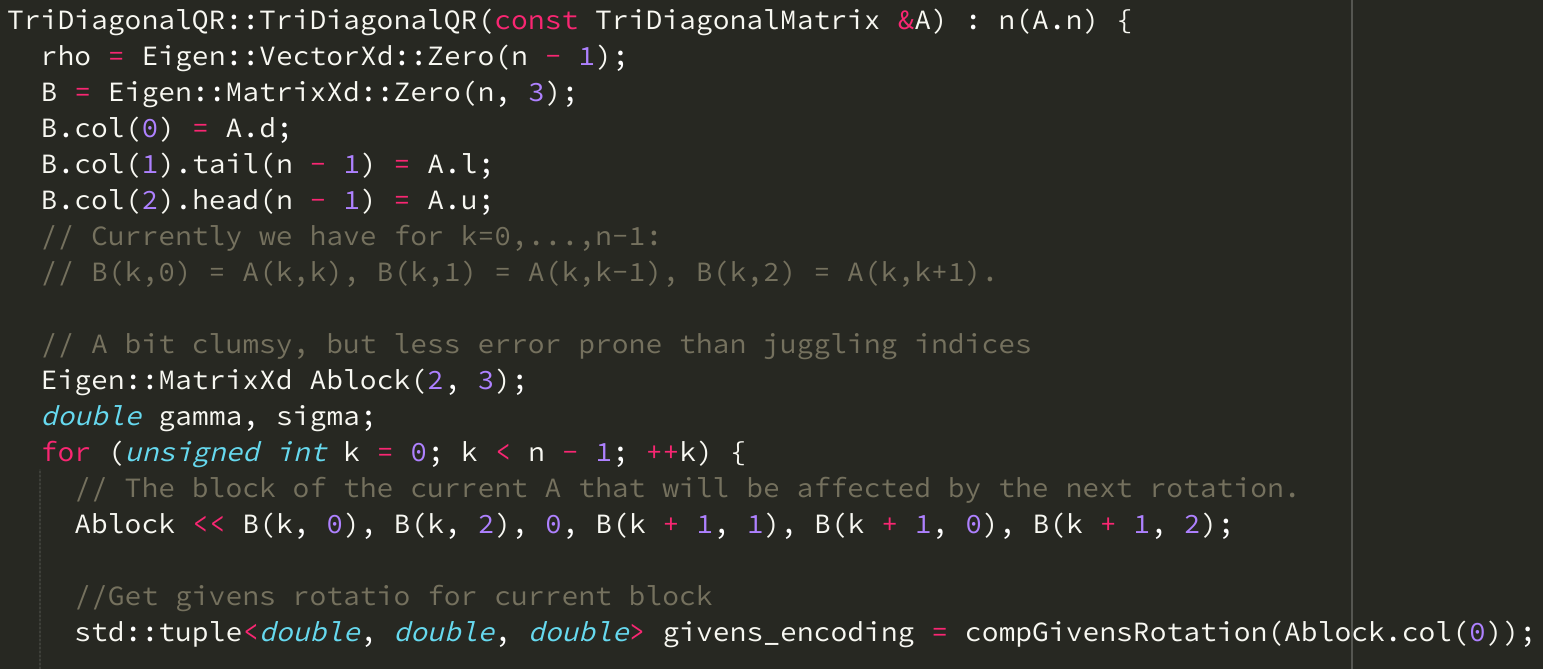
\includegraphics[width=1.0\linewidth]{3-4.c_1.png}
\end{figure}

\pagebreak 

\begin{figure}[!hbt]
    \centering
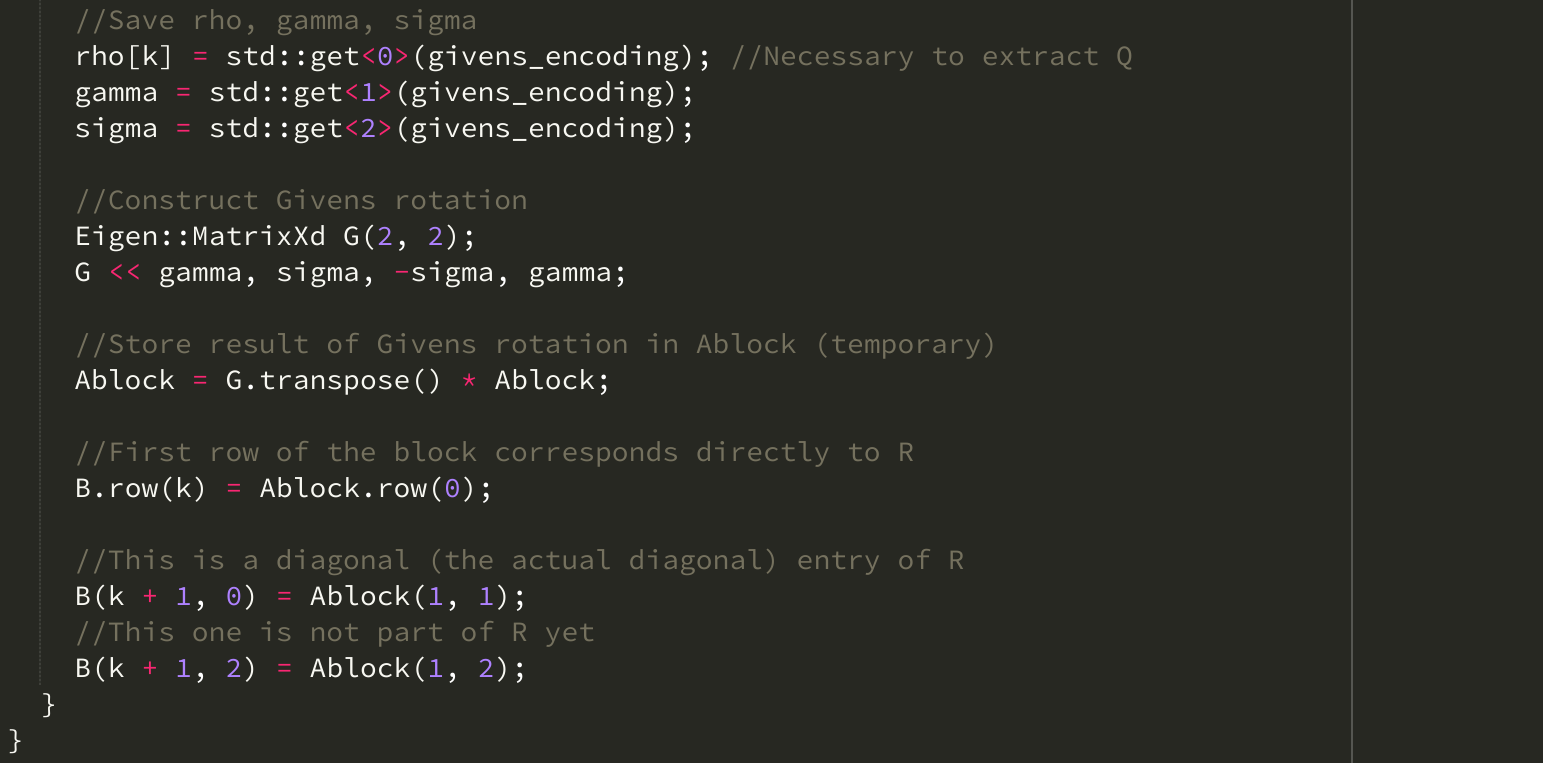
\includegraphics[width=1.0\linewidth]{3-4.c_2.png}
\end{figure}

\subsection*{3-4.d}
We are tasked with implementing (efficiently) the method \verb|applyQT| of the \verb|TriDiagonalQR| class which computes $\mathbf{Q}^{\mathsf{T}}\mathbf{x} = \mathbf{Q}^{-1}\mathbf{x}$ for a given vector $\mathbf{x}\in \mathbb{R}^{n}$. When \verb|applyQT| is called we now that we have already initialized the instance of the class and hence all rotation values $\rho$ are computed, as well as the matrix $\mathbf{R}$ in \verb|B|. We are already given a method that computes the Givens-Rotation in the form of \verb|Givens|. The hint tells us to look at code segment 3.3.4.5, but it is as unreadable as it comes. The most important things to note are
\begin{itemize}
    \item The matrix \verb|R| is named suboptimal at most, as it is the Givens rotation matrix and not the matrix $\mathbf{R}$ of the decomposition.
    \item The line of code \verb|b.segment(k,2).applyOnTheLeft(R)| does \verb|R * b.segment(k, 2)| and stores it in again in \verb|b.segment(k,2)|. This is done in the hopes that the Eigen internal implementation will not create a temporary object when computing the result. We will use the normal multiplication.
\end{itemize}
What we do now is for each adjacent entries of \verb|x| we perform the corresponding Givens-Rotation, where this corresponds overall with multiplying by $\mathbf{Q}^{\mathsf{T}}$. The transposed comes from the fact that  we have $\mathbf{Q}^{\mathsf{T}}\mathbf{A}= \mathbf{R}$ which is how the rotations are done (not by multiplying with $\mathbf{Q}$ but the effect is the same). 

\pagebreak

\noindent This gives us the following code.
\begin{figure}[!hbt]
    \centering
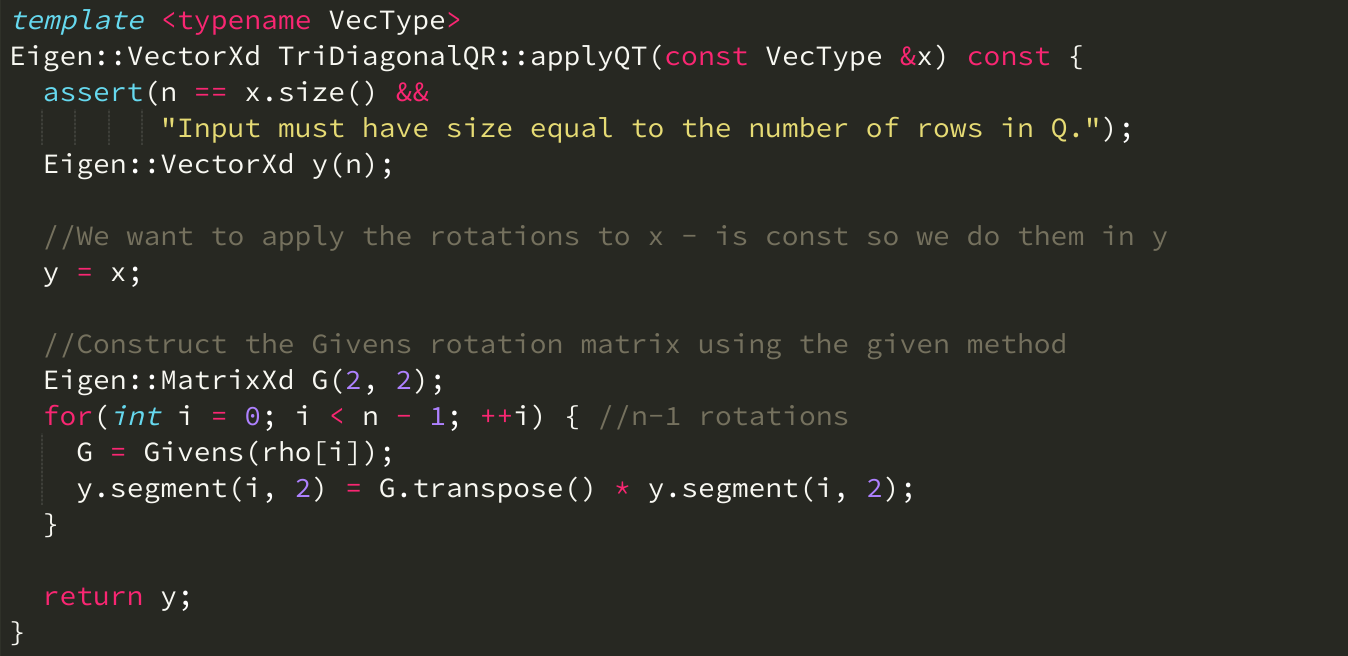
\includegraphics[width=1.0\linewidth]{3-4.d.png}
\end{figure}

\subsection*{3-4.e}
We are now tasked with efficiently implementing the method \verb|solve| of \verb|TriDiagonalQR| that accepts a vector $\mathbf{b}\in \mathbb{R}^{n}$ as argument and then solves the linear systems of equations $\mathbf{A}\mathbf{x}=\mathbf{b}$, where $\mathbf{A}$ is the tridiagonal matrix stored in the current \verb|TriDiaagonalQR| obejct. If $\mathbf{A}$ is not invertible then a \verb|std::runtime_error| exception should be thrown. Let us look at how we will solve the given LSE $\mathbf{A}\mathbf{x} = \mathbf{b}$ using its QR-decomposition. We have
\begin{equation*}
    \mathbf{A}\mathbf{x} = \mathbf{Q}\mathbf{R}\mathbf{x} = \mathbf{b}
\end{equation*}
We hence have two systems to solve
\begin{equation*}
    \mathbf{Q}\mathbf{c} = \mathbf{b} \text{ with } \mathbf{c} = \mathbf{R}\mathbf{x}
\end{equation*}
this we can simply solve by using that $\mathbf{Q}$ is orthogonal and hence we get $\mathbf{c} = \mathbf{Q}^{\mathsf{T}}\mathbf{b}$. We have already implemented a method that can do this (\verb|applyQT|). The second system is given by
\begin{equation*}
    \mathbf{R}\mathbf{x} = \mathbf{c}
\end{equation*}
and because $\mathbf{R}$ is upper triangular we can use backwards substitution to solve this. $\mathbf{R}$ is what determines if $\mathbf{A}$ is invertible or not and this only depends on all diagonal entries being non-zero, as otherwise the determinant of $\mathbf{R}$ is zero (\mathbf{R} is triangular) and thus $\mathbf{R}$ would not be invertible and the system could not be solved. First this function is given to us.

\pagebreak

\noindent This gives us the following code.

\begin{figure}[!hbt]
    \centering
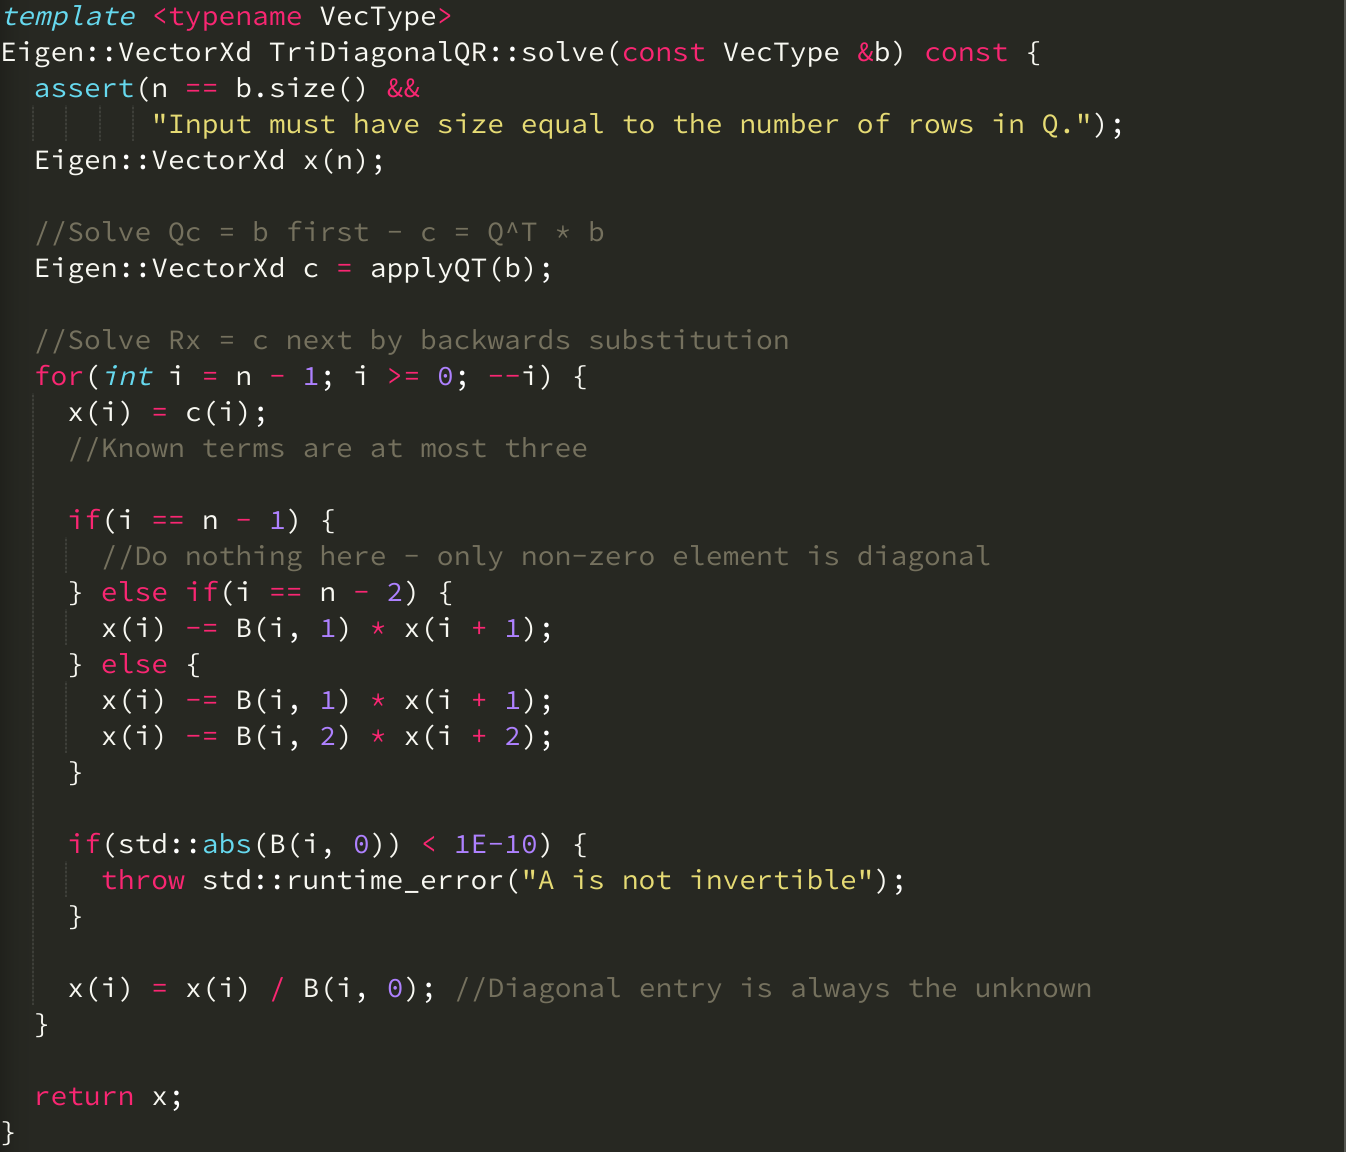
\includegraphics[width=1.0\linewidth]{3-4.e.png}
\end{figure}
\subsection*{3-4.f}
We are tasked with giving the asymptotic complexity of the constructor of \verb|TriDiagonalQR|, \verb|applyQT| and \verb|solve|. The constructor applies $n-1$ Givens rotations to $3$ vectors each time and hence takes $\mathcal{O}\left(n\right)$ time. The \verb|applyQT| function applies $n-1$ Givens rotations to segments of \verb|x|, this takes $\mathcal{O}\left(n\right)$ time overall. The \verb|solve| function calls \verb|applyQT| which adds $\mathcal{O}\left(n\right)$ to the computational cost, then backwards substitution does $n-1$ computations which each have at most $\mathcal{O}\left(1\right)$ computational cost. We hence also get $\mathcal{O}\left(n\right)$ overall.

\pagebreak

\subsection*{3-4.g}
We are tasked with implementing a specialization of the given code for the \textbf{inverse iteration} (Chapter 9). The following code is given to us.
\begin{figure}[!hbt]
    \centering
\includegraphics[width=1.0\linewidth]{InverseIteration.png}
\end{figure}

\noindent The main problem with the code is that we would want to use our own specialized QR-decomposition based solving utility. This requires only little change, which produces the following code.

\begin{figure}[!hbt]
    \centering
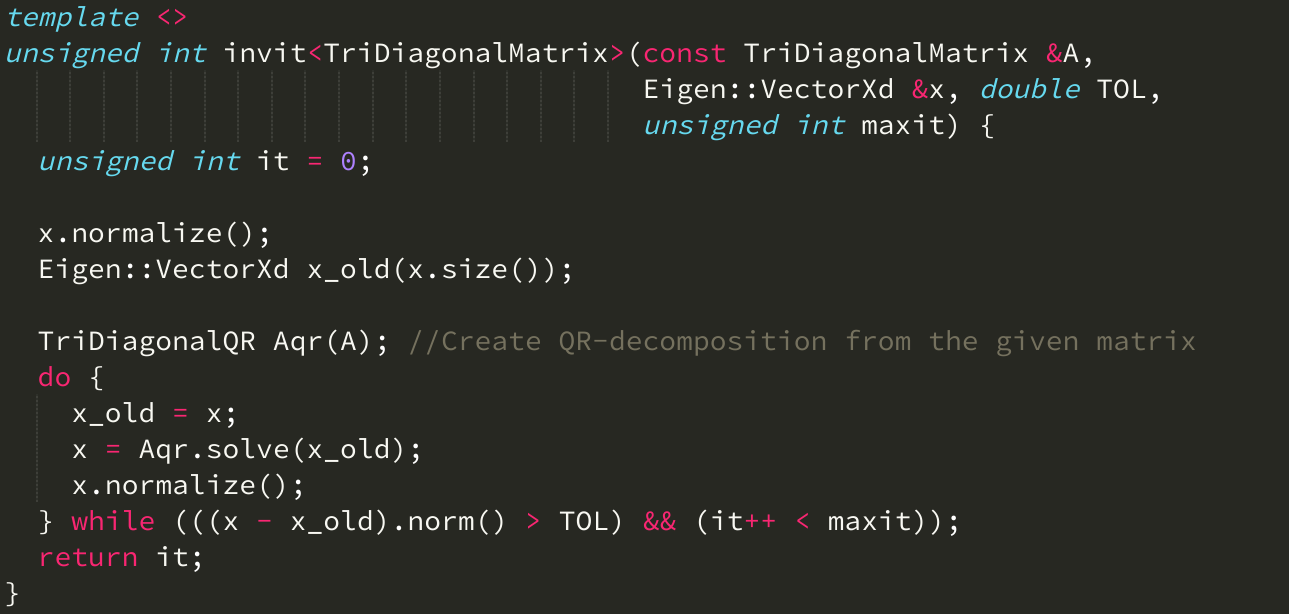
\includegraphics[width=1.0\linewidth]{3-4.g.png}
\end{figure}

\end{document}
